\documentclass[11pt,a4paper]{article}

\usepackage[
    a4paper,
    left=15mm,
    right=15mm,
    top=30mm,
    bottom=25mm,
    headheight=25mm
]{geometry}
\usepackage{graphicx}
\usepackage{polski}
\usepackage[utf8]{inputenc}
\usepackage{enumerate}
\usepackage{comment}
\usepackage{fancyhdr}
\usepackage{hyperref}
\usepackage{indentfirst}
\usepackage{multirow}
\usepackage{multicol}
\usepackage{float}
\usepackage{amsmath}
\usepackage{amssymb}
\usepackage{wrapfig}
\usepackage{layout}
\usepackage{textcomp}
\usepackage[center]{caption}
\usepackage{subcaption}
\usepackage{siunitx}
\usepackage[mathscr]{euscript}
\usepackage{xcolor,colortbl}
\usepackage{setspace}
\usepackage{algorithm}
\usepackage[rightComments=false]{algpseudocodex}
\usepackage{listings}
\usepackage{amsthm}
\usepackage{needspace}

% no lone first/last lines of a paragraph on a page
\widowpenalty=10000
\clubpenalty=10000
\displaywidowpenalty=10000

\sisetup{output-exponent-marker=\ensuremath{\mathrm{e}}, output-decimal-marker={,}}
\algrenewcommand\algorithmicprocedure{\textbf{Procedura}}
\algrenewcommand\algorithmicfor{\textbf{Dla}}
\algrenewcommand\algorithmicdo{\textbf{powtarzaj}}
\algrenewcommand\algorithmicwhile{\textbf{Dopóki}}
\algrenewcommand\algorithmicloop{\textbf{Powtarzaj}}
\algrenewcommand\algorithmicif{\textbf{Jeżeli}}
\algrenewcommand\algorithmicelse{\textbf{Inaczej}}
\algrenewcommand\algorithmicthen{\textbf{wykonaj}}
\algrenewcommand\algorithmicend{\textbf{Koniec}}
\algrenewcommand\algorithmicreturn{\textbf{zwróć}}

\newenvironment{algorytm}[1][htb]
  {\par\bigskip\floatname{algorithm}{}\renewcommand{\thealgorithm}{}
   \begin{algorithm}[#1]%
  }{\end{algorithm}\par\bigskip}

\renewcommand{\baselinestretch}{1.18}
\renewcommand\thesubfigure{\roman{subfigure}}

\renewcommand\lstlistingname{Kod}
\lstset{
    language=Java,
    basicstyle=\ttfamily\footnotesize,
    keywordstyle=\bfseries,
    commentstyle=\itshape\color{gray},
    numbers=left,
    numberstyle=\tiny\color{gray},
    numbersep=8pt,
    frame=tb,
    xleftmargin=6mm,
    columns=fullflexible,
    keepspaces=true,
    showstringspaces=false,
    tabsize=4,
    captionpos=b,
    breaklines=true,
    postbreak=\mbox{\textcolor{gray}{$\hookrightarrow$}\space}
}

\pagestyle{fancy}
\fancyhead[L]{
    
\includegraphics[height=12mm]{img/agh-logo.jpg}
}
\fancyhead[R]{}

\author{Szymon Iwaniuk}
\title{
    
\includegraphics[height=45mm]{img/agh-logo.jpg}
    \vspace{10mm}
    \\
    Problem czytelników i pisarzy}
\date{Teoria Współbieżności 2025/2026, laboratorium 6 \\ 16 listopada 2026}

\begin{document}

\maketitle
\tableofcontents
\pagebreak

\section{Wstęp}
\subsection{Treść zadania}
\textbf{Zadanie 1 -- problem czytelników i pisarzy.} Problem czytelników i pisarzy proszę rozwiązać
przy pomocy semaforów i zmiennych warunkowych. Proszę wykonać pomiary dla różnej liczby czytelników
(10--100) i pisarzy (od 1 do 10). W sprawozdaniu proszę narysować trójwymiarowy wykres czasu
w zależności od liczby wątków i go zinterpretować.

Założenia problemu: z czytelni może jednocześnie korzystać wielu czytelników, ale jeśli przebywa w niej
pisarz, żaden inny proces nie może do niej wejść. Każdy czytelnik i każdy pisarz, który chce wejść,
w końcu wejdzie (warunek żywotności).

\textbf{Zadanie 2 -- blokowanie drobnoziarniste.}
\begin{enumerate}
    \item Proszę zaimplementować listę, w której każdy węzeł składa się z wartości typu \texttt{Object},
          referencji do następnego węzła oraz zamka (\texttt{lock}).
    \item Proszę zastosować metodę drobnoziarnistego blokowania do metod
          \texttt{boolean contains(Object o)}, \texttt{boolean remove(Object o)} (usuwa pierwsze
          wystąpienie) oraz \texttt{boolean add(Object o)} (dodaje na końcu listy).
    \item Proszę porównać wydajność tego rozwiązania w stosunku do listy z jednym zamkiem blokującym
          dostęp do całości. Należy założyć, że koszt czasowy operacji na elemencie listy (porównanie,
          wstawianie obiektu) może być duży -- proszę wykonać pomiary dla różnych wartości tego kosztu.
\end{enumerate}
Podczas przeglądania listy zamykamy zamek na pierwszym elemencie, potem na drugim, otwieramy zamek
na pierwszym, zamykamy na trzecim, otwieramy na drugim i tak dalej. Dzięki temu nie blokujemy całej
listy i wiele wątków może jednocześnie przeglądać i modyfikować różne jej fragmenty.

\subsection{Opis rozwiązania}
W zadaniu 1 porównujemy trzy implementacje czytelni:
\begin{itemize}
    \item \textbf{semafory} -- klasyczne rozwiązanie z dwoma semaforami binarnymi i licznikiem czytelników;
          czytelnicy mają pierwszeństwo, więc pisarze mogą zostać zagłodzeni,
    \item \textbf{semafory z kołowrotem} -- to samo rozwiązanie z dodatkowym sprawiedliwym semaforem
          (kołowrotem), przez który przechodzą wszyscy; usuwa zagłodzenie pisarzy,
    \item \textbf{zmienne warunkowe} -- \texttt{ReentrantLock} z warunkami \textit{okToRead} i \textit{okToWrite};
          nowy czytelnik czeka, gdy czeka pisarz, a wychodzący pisarz wpuszcza wszystkich czekających
          czytelników naraz.
\end{itemize}
W zadaniu 2 porównujemy listę z blokowaniem drobnoziarnistym z listą z jednym zamkiem.
Razem ze sprawozdaniem zawarty jest kod w języku \texttt{Java}, program wykonujący pomiary
oraz skrypt generujący wykresy.

\section{Specyfikacja narzędzi i sprzętu}
Program został napisany w języku \texttt{Java 27} i uruchomiony na maszynie wirtualnej
\texttt{OpenJDK}, na komputerze z procesorem \texttt{Apple M4} (architektura \texttt{ARM64},
10 rdzeni: 4 wydajnościowe i 6 energooszczędnych), \texttt{16 GB} zunifikowanej pamięci
\texttt{LPDDR5} i systemem operacyjnym \texttt{macOS 26}.
Do wygenerowania wykresów użyty został \texttt{Python} z biblioteką \texttt{matplotlib}.

\subsection{Metoda pomiaru}
Wszystkie wątki startują jednocześnie po zwolnieniu zatrzasku \texttt{CountDownLatch}, a czas mierzymy
zegarem \texttt{System.nanoTime()} od startu do zakończenia ostatniego wątku. Przed pomiarami wykonujemy
przebiegi rozgrzewające kompilator JIT, a każdą konfigurację uruchamiamy trzy razy i bierzemy medianę.

\textbf{Zadanie 1.} Każdy czytelnik wykonuje 20 odczytów, a każdy pisarz 20 zapisów. Przed każdym
wejściem wątek ,,myśli'' średnio 1 ms, odczyt i zapis trwają średnio 0,2 ms (czasy losowane jednostajnie
z $[0, 2t)$, opóźnienie przez \texttt{LockSupport.parkNanos}). Mierzymy czas całego przebiegu oraz
czas oczekiwania na wejście do czytelni, osobno dla czytelników i pisarzy. Parametry: czytelnicy
$\in \{10, 20, \dots, 100\}$, pisarze $\in \{1, \dots, 10\}$. W czytelni sprawdzamy licznikami atomowymi,
że pisarz jest zawsze sam -- naruszenie przerwałoby pomiary wyjątkiem.

\textbf{Zadanie 2.} Lista zawiera na początku klucze $0, \dots, 99$. Każdy wątek wykonuje swoją część
ustalonej liczby operacji na losowym kluczu z tego zakresu: 60\% \texttt{contains}, 20\% \texttt{add},
20\% \texttt{remove}. Koszt operacji na elemencie (każde porównanie i wstawienie) symulujemy aktywnym
oczekiwaniem przez $c \in \{0;\ 0{,}1;\ 1;\ 10\}$ \textmu s. Liczba wątków: 1, 2, 4, 8.
Wynikiem jest przepustowość (operacje na sekundę). Po każdym przebiegu sprawdzamy, że rozmiar listy
jest równy $100 + \text{dodane} - \text{usunięte}$ i że żaden zamek węzła nie pozostał zajęty.

\section{Zadanie 1 -- czytelnicy i pisarze}
\subsection{Algorytmy}
\needspace{16\baselineskip}
\textbf{Semafory.} Semafor \textit{mutex} chroni licznik czytelników $r$, a semafor \textit{w}
jest zajęty przez pisarza albo przez całą grupę czytelników.

\begin{algorytm}[H]
\setstretch{1.35}
\begin{algorithmic}[1]
    \Procedure{startRead}{}
        \State \textsc{P}(\textit{mutex}); \ $r \gets r + 1$
        \If{$r = 1$} \textsc{P}(\textit{w}) \Comment{pierwszy czytelnik blokuje pisarzy}
        \EndIf
        \State \textsc{V}(\textit{mutex})
    \EndProcedure
    \Procedure{endRead}{}
        \State \textsc{P}(\textit{mutex}); \ $r \gets r - 1$
        \If{$r = 0$} \textsc{V}(\textit{w}) \Comment{ostatni czytelnik wpuszcza pisarzy}
        \EndIf
        \State \textsc{V}(\textit{mutex})
    \EndProcedure
    \Procedure{startWrite}{} \ \textsc{P}(\textit{w})
    \EndProcedure
    \Procedure{endWrite}{} \ \textsc{V}(\textit{w})
    \EndProcedure
\end{algorithmic}
\caption{Czytelnicy i pisarze na semaforach}
\end{algorytm}

Dopóki w czytelni jest choć jeden czytelnik, kolejni wchodzą bez czekania. Jeżeli czytelnicy
przychodzą na tyle często, że $r$ nie spada do zera, pisarz czeka w nieskończoność (zagłodzenie pisarzy).

\needspace{12\baselineskip}
\textbf{Semafory z kołowrotem.} Dodajemy sprawiedliwy semafor \textit{t} (FIFO).
Pisarz trzyma go, czekając na \textit{w}, więc czytelnicy, którzy przyszli po nim, czekają za nim.

\begin{algorytm}[H]
\setstretch{1.35}
\begin{algorithmic}[1]
    \Procedure{startRead}{}
        \State \textsc{P}(\textit{t}); \ \textsc{V}(\textit{t}); \ dalej jak w wierszach 2--4 rozwiązania z semaforami
    \EndProcedure
    \Procedure{startWrite}{}
        \State \textsc{P}(\textit{t}); \ \textsc{P}(\textit{w}); \ \textsc{V}(\textit{t})
    \EndProcedure
\end{algorithmic}
\caption{Kołowrót (\textsc{endRead} i \textsc{endWrite} bez zmian)}
\end{algorytm}

\needspace{30\baselineskip}
\textbf{Zmienne warunkowe.} Stan czytelni: $r$ -- czytelnicy w środku, \textit{pisze} -- czy jest pisarz,
$c_r$, $c_w$ -- liczba czekających czytelników i pisarzy, \textit{tura} -- numer wpuszczenia grupy czytelników.

\begin{algorytm}[H]
\setstretch{1.35}
\begin{algorithmic}[1]
    \Procedure{startRead}{} \Comment{wszystkie procedury pod zamkiem}
        \If{$\textit{pisze} \lor c_w > 0$}
            \State $c_r \gets c_r + 1$, \ $t \gets \textit{tura}$
            \While{$t = \textit{tura}$} \ \textsc{await}(\textit{okToRead})
            \EndWhile
            \State \Return \Comment{pisarz już doliczył nas do $r$}
        \EndIf
        \State $r \gets r + 1$
    \EndProcedure
    \Procedure{endRead}{}
        \State $r \gets r - 1$
        \If{$r = 0 \land c_w > 0$} \textsc{signal}(\textit{okToWrite})
        \EndIf
    \EndProcedure
    \Procedure{startWrite}{}
        \State $c_w \gets c_w + 1$
        \While{$\textit{pisze} \lor r > 0$} \ \textsc{await}(\textit{okToWrite})
        \EndWhile
        \State $c_w \gets c_w - 1$, \ $\textit{pisze} \gets \texttt{true}$
    \EndProcedure
    \Procedure{endWrite}{}
        \State $\textit{pisze} \gets \texttt{false}$
        \If{$c_r > 0$}
            \State $r \gets r + c_r$, \ $c_r \gets 0$, \ $\textit{tura} \gets \textit{tura} + 1$, \ \textsc{signalAll}(\textit{okToRead})
        \Else
            \State \textsc{signal}(\textit{okToWrite})
        \EndIf
    \EndProcedure
\end{algorithmic}
\caption{Czytelnicy i pisarze na zmiennych warunkowych}
\end{algorytm}

Pisarz nie jest głodzony, bo czytelnicy przychodzący po nim czekają (wiersz 2). Czytelnicy nie są
głodzeni, bo każdy wychodzący pisarz wpuszcza wszystkich czekających czytelników (wiersz 17),
zanim wejdzie kolejny pisarz. Pisarz w wierszu 17 sam zwiększa $r$ o liczbę wpuszczonych
czytelników -- gdyby robili to obudzeni czytelnicy, inny pisarz mógłby zdobyć zamek przed nimi,
zobaczyć $r = 0$ i wejść razem z nimi. Licznik \textit{tura} chroni przed fałszywymi pobudkami.

\subsection{Implementacja}
Każde rozwiązanie dziedziczy po klasie \textbf{ReadingRoom} z metodami \texttt{startRead},
\texttt{endRead}, \texttt{startWrite} i \texttt{endWrite}. Poniżej znajdują się klasy z semaforami
i ze zmiennymi warunkowymi. Klasa \textbf{FairSemaphoreRW} różni się od \textbf{SemaphoreRW} tylko
kołowrotem opisanym w rozdziale 3.1, a pełny kod (wraz z programem pomiarowym) znajduje się w katalogu \texttt{src}.

\begin{lstlisting}[caption={Klasa \textbf{SemaphoreRW} (\texttt{src/SemaphoreRW.java})}]
import java.util.concurrent.Semaphore;

/** Classic semaphore solution with reader preference: writers can starve while readers keep coming. */
class SemaphoreRW extends ReadingRoom {
    private final Semaphore mutex = new Semaphore(1);     // protects readCount
    private final Semaphore writeLock = new Semaphore(1); // held by a writer or by the group of readers
    private int readCount = 0;

    @Override
    void startRead() throws InterruptedException {
        mutex.acquire();
        if (++readCount == 1) writeLock.acquire(); // first reader locks out writers
        mutex.release();
    }

    @Override
    void endRead() {
        mutex.acquireUninterruptibly();
        if (--readCount == 0) writeLock.release(); // last reader lets writers in
        mutex.release();
    }

    @Override
    void startWrite() throws InterruptedException {
        writeLock.acquire();
    }

    @Override
    void endWrite() {
        writeLock.release();
    }
}
\end{lstlisting}

\begin{lstlisting}[caption={Klasa \textbf{ConditionRW} (\texttt{src/ConditionRW.java})}]
import java.util.concurrent.locks.Condition;
import java.util.concurrent.locks.ReentrantLock;

/**
 * Condition variables. A new reader waits while a writer is waiting, and a writer that leaves
 * lets in all readers waiting at that moment, so neither readers nor writers starve.
 */
class ConditionRW extends ReadingRoom {
    private final ReentrantLock lock = new ReentrantLock();
    private final Condition okToRead = lock.newCondition();
    private final Condition okToWrite = lock.newCondition();
    private int readers = 0, waitingReaders = 0, waitingWriters = 0;
    private boolean writing = false;
    private long readTurn = 0; // changes when a writer admits the waiting readers

    @Override
    void startRead() throws InterruptedException {
        lock.lock();
        try {
            if (writing || waitingWriters > 0) {
                waitingReaders++;
                long turn = readTurn;
                while (turn == readTurn) okToRead.await();
                return; // the writer already counted us in readers
            }
            readers++;
        } finally {
            lock.unlock();
        }
    }

    @Override
    void endRead() {
        lock.lock();
        try {
            if (--readers == 0 && waitingWriters > 0) okToWrite.signal();
        } finally {
            lock.unlock();
        }
    }

    @Override
    void startWrite() throws InterruptedException {
        lock.lock();
        try {
            waitingWriters++;
            while (writing || readers > 0) okToWrite.await();
            waitingWriters--;
            writing = true;
        } finally {
            lock.unlock();
        }
    }

    @Override
    void endWrite() {
        lock.lock();
        try {
            writing = false;
            if (waitingReaders > 0) { // admit the whole group of waiting readers
                readers += waitingReaders;
                waitingReaders = 0;
                readTurn++;
                okToRead.signalAll();
            } else {
                okToWrite.signal();
            }
        } finally {
            lock.unlock();
        }
    }
}
\end{lstlisting}

\subsection{Wyniki}
\textbf{Rysunek 1} pokazuje czas wykonania w zależności od liczby czytelników i pisarzy,
a \textbf{rysunek 2} średni czas oczekiwania na wejście do czytelni.

\begin{figure}[H]
    \centering
    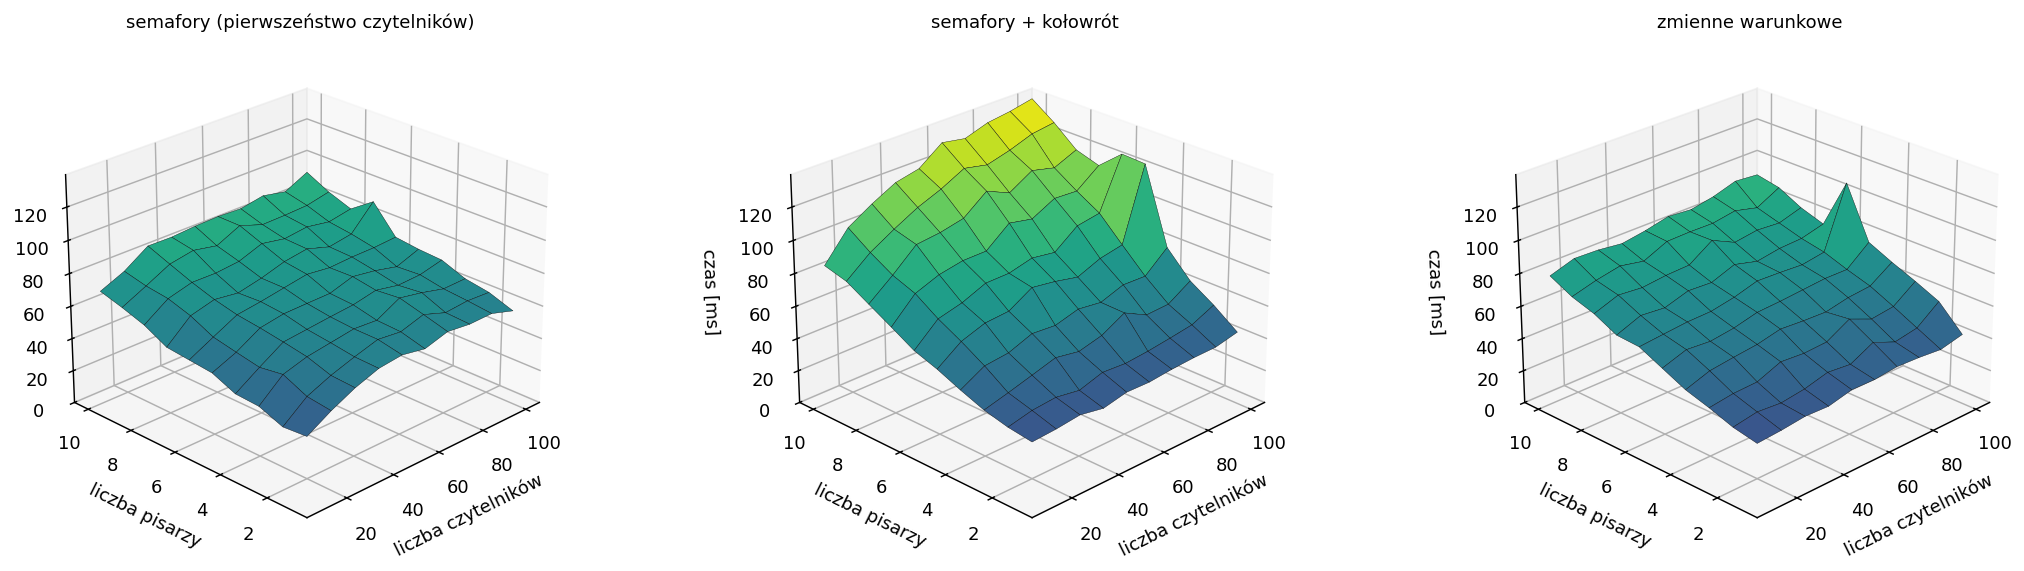
\includegraphics[width=\textwidth]{img/rw_time.png}
    \caption{Czas wykonania w zależności od liczby czytelników i pisarzy}
\end{figure}

\begin{figure}[H]
    \centering
    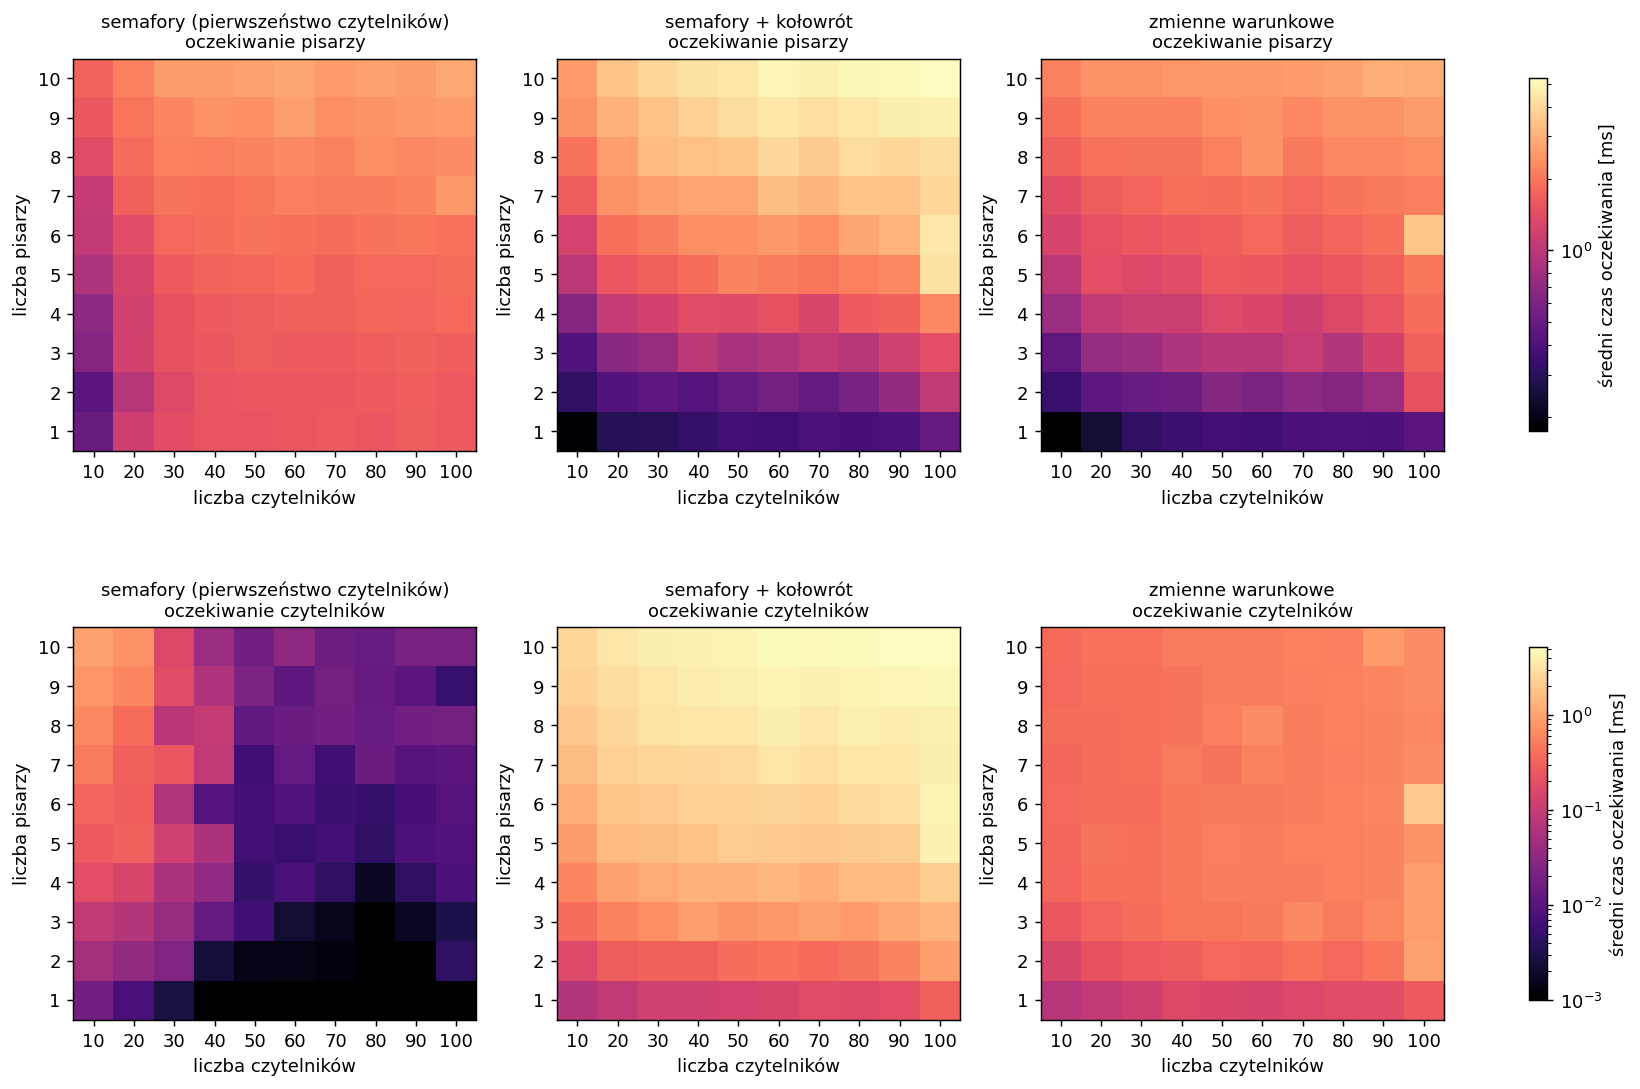
\includegraphics[width=\textwidth]{img/rw_wait.png}
    \caption{Średni czas oczekiwania pisarzy (u góry) i czytelników (u dołu), skala logarytmiczna}
\end{figure}

\textbf{Tabela 1} zestawia mediany w narożnikach badanego zakresu.

\begin{table}[H]
    \centering
    \renewcommand{\arraystretch}{1.25}
    \begin{tabular}{|l|r|r|r|r|r|}
        \hline
        \textbf{Rozwiązanie} & \textbf{czyt.} & \textbf{pis.} & \textbf{czas [ms]} & \textbf{oczek. czyt. [ms]} & \textbf{oczek. pis. (maks.) [ms]} \\ \hline
        \multirow{4}{*}{semafory} & 10 & 1 & \num{39.1} & \num{0.02} & \num{0.51} (\num{2.9}) \\ \cline{2-6}
         & 100 & 1 & \num{57.2} & \num{0.00} & \num{1.60} (\num{31.8}) \\ \cline{2-6}
         & 10 & 10 & \num{69.2} & \num{0.98} & \num{1.72} (\num{4.2}) \\ \cline{2-6}
         & 100 & 10 & \num{93.0} & \num{0.02} & \num{2.82} (\num{32.8}) \\ \hline
        \multirow{4}{*}{semafory + kołowrót} & 10 & 1 & \num{35.8} & \num{0.07} & \num{0.18} (\num{0.5}) \\ \cline{2-6}
         & 100 & 1 & \num{44.1} & \num{0.30} & \num{0.50} (\num{1.0}) \\ \cline{2-6}
         & 10 & 10 & \num{84.8} & \num{2.57} & \num{2.58} (\num{4.4}) \\ \cline{2-6}
         & 100 & 10 & \num{139.1} & \num{5.20} & \num{5.26} (\num{7.0}) \\ \hline
        \multirow{4}{*}{zmienne warunkowe} & 10 & 1 & \num{35.0} & \num{0.07} & \num{0.17} (\num{0.5}) \\ \cline{2-6}
         & 100 & 1 & \num{42.6} & \num{0.27} & \num{0.45} (\num{0.9}) \\ \cline{2-6}
         & 10 & 10 & \num{78.6} & \num{0.37} & \num{2.17} (\num{11.9}) \\ \cline{2-6}
         & 100 & 10 & \num{91.4} & \num{0.66} & \num{2.91} (\num{17.6}) \\ \hline
    \end{tabular}
    \caption{Czas wykonania i czasy oczekiwania (średni, w nawiasie maksymalny)}
\end{table}

Czas rośnie przede wszystkim z liczbą pisarzy. Pisarze wchodzą pojedynczo, więc sama ich praca
(20 zapisów po średnio 0,2 ms) daje dla 10 pisarzy co najmniej 40 ms wyłącznego dostępu.
Czytelnicy czytają równolegle, więc ich liczba wpływa na czas słabiej. W rozwiązaniach z kołowrotem
i ze zmiennymi warunkowymi zwiększenie liczby pisarzy z 1 do 10 wydłuża przebieg o 106--242\%,
a zwiększenie liczby czytelników z 10 do 100 o 16--136\%. W rozwiązaniu z semaforami oba wpływy są
podobne (37--77\% i 31--69\%), bo pisarze i tak czekają, aż czytelnicy przestaną przychodzić.

W rozwiązaniu z semaforami czytelnicy prawie nie czekają (dla 100 czytelników średnio najwyżej 0,02 ms),
ale pisarze czekają najdłużej: dla 100 czytelników i jednego pisarza najdłuższe oczekiwanie wynosi
31,8 ms przy całym przebiegu trwającym 57 ms, a w całym zakresie do 36,3 ms. To zagłodzenie
pisarzy przez czytelników -- przy stałym napływie czytelników $r$ długo nie spada do zera.
Przez to przebieg trwa dłużej niż w pozostałych rozwiązaniach (57 ms wobec 43--44 ms), bo pisarz
kończy pracę dopiero, gdy czytelnicy przestaną przychodzić.

Kołowrót usuwa zagłodzenie: najdłuższe oczekiwanie pisarza spada do 8,6 ms w całym zakresie, a średnie
czasy oczekiwania czytelników i pisarzy są prawie równe (5,20 i 5,26 ms dla 100 czytelników i 10 pisarzy).
Ceną jest wydajność: wszyscy przechodzą przez jeden semafor w kolejności przyjścia, więc każdy pisarz
rozdziela czytelników na małe grupy i przebieg dla 100 czytelników i 10 pisarzy trwa 139 ms.

Zmienne warunkowe łączą zalety obu rozwiązań. Wychodzący pisarz wpuszcza naraz wszystkich czekających
czytelników, więc czytelnicy czekają krótko (0,66 ms dla 100 czytelników i 10 pisarzy), a pisarz nie jest
głodzony (najdłużej 21,6 ms w całym zakresie, mniej niż w rozwiązaniu z semaforami). Czas
dla 100 czytelników i 10 pisarzy (91 ms) jest taki jak w rozwiązaniu z semaforami. Najdłuższe oczekiwania
pisarzy są tu dłuższe niż z kołowrotem, bo \texttt{ReentrantLock} nie jest sprawiedliwy między pisarzami:
\textsc{signal} budzi jednego z nich, a zamek może przejąć inny.

\subsection{Wnioski}
O czasie wykonania decyduje przede wszystkim liczba pisarzy, bo ich praca jest szeregowana,
a czytelnicy czytają równolegle (wyjątkiem jest rozwiązanie z pierwszeństwem czytelników). Klasyczne rozwiązanie na semaforach jest najprostsze
i daje czytelnikom najkrótsze czasy oczekiwania, ale głodzi pisarzy. Kołowrót zapewnia sprawiedliwość
kosztem równoległości czytelników. Rozwiązanie na zmiennych warunkowych nie głodzi żadnej grupy
i zachowuje grupowe wpuszczanie czytelników, dlatego jest najlepszym kompromisem.

\section{Zadanie 2 -- blokowanie drobnoziarniste}
\subsection{Algorytmy}
Lista ma węzeł-wartownika \textit{head}, który nigdy nie jest usuwany. Wątek trzyma w każdej chwili
co najwyżej dwa sąsiednie zamki i zamyka następny węzeł, zanim otworzy poprzedni, więc żaden
inny wątek nie może go wyprzedzić ani zmienić odcinka, na którym pracuje. $\textsc{work}()$ oznacza
kosztowną operację na elemencie (porównanie lub wstawienie).

\needspace{26\baselineskip}
\begin{algorytm}[H]
\setstretch{1.35}
\begin{algorithmic}[1]
    \Procedure{contains}{$o$}
        \State $p \gets \textit{head}$, \ \textsc{lock}($p$), \ $c \gets p.\textit{next}$
        \While{$c \ne \texttt{null}$}
            \State \textsc{lock}($c$), \ \textsc{unlock}($p$), \ \textsc{work}()
            \If{$c.\textit{value} = o$} \textsc{unlock}($c$), \Return \texttt{true}
            \EndIf
            \State $p \gets c$, \ $c \gets c.\textit{next}$
        \EndWhile
        \State \textsc{unlock}($p$), \Return \texttt{false}
    \EndProcedure
    \Procedure{remove}{$o$}
        \State $p \gets \textit{head}$, \ \textsc{lock}($p$), \ $c \gets p.\textit{next}$
        \While{$c \ne \texttt{null}$}
            \State \textsc{lock}($c$), \ \textsc{work}() \Comment{zamknięte $p$ i $c$}
            \If{$c.\textit{value} = o$}
                \State $p.\textit{next} \gets c.\textit{next}$, \ \textsc{unlock}($c$), \ \textsc{unlock}($p$), \Return \texttt{true}
            \EndIf
            \State \textsc{unlock}($p$), \ $p \gets c$, \ $c \gets c.\textit{next}$
        \EndWhile
        \State \textsc{unlock}($p$), \Return \texttt{false}
    \EndProcedure
    \Procedure{add}{$o$}
        \State $p \gets \textit{head}$, \ \textsc{lock}($p$)
        \While{$p.\textit{next} \ne \texttt{null}$}
            \State $n \gets p.\textit{next}$, \ \textsc{lock}($n$), \ \textsc{unlock}($p$), \ $p \gets n$, \ \textsc{work}()
        \EndWhile
        \State \textsc{work}(), \ $p.\textit{next} \gets$ nowy węzeł($o$), \ \textsc{unlock}($p$), \Return \texttt{true}
    \EndProcedure
\end{algorithmic}
\caption{Lista z blokowaniem drobnoziarnistym}
\end{algorytm}

W \textsc{remove} usuwany węzeł $c$ i jego poprzednik $p$ są zamknięte jednocześnie (wiersz 13), więc
nikt nie może w tym czasie zmienić $p.\textit{next}$ ani przejść przez $c$. W \textsc{contains}
wystarczy jeden zamek przy porównaniu, ale przejście do następnego węzła wymaga zamknięcia go przed
otwarciem bieżącego. W \textsc{add} ostatni węzeł jest zamknięty podczas dopisywania, więc dwa wątki
nie mogą dopisać elementu w to samo miejsce. Łatwo tu o błędy: przejście dalej bez zamka na następnym
węźle albo dwukrotne otwarcie tego samego zamka (np. w bloku \texttt{finally}). Dlatego po każdym
przebiegu sprawdzamy rozmiar listy i to, że żaden zamek nie pozostał zajęty.
Lista z jednym zamkiem wykonuje te same pętle bez zamków węzłów, a całe metody są sekcją krytyczną.

\subsection{Implementacja}
\begin{lstlisting}[caption={Klasa \textbf{FineList} (\texttt{src/FineList.java})}]
import java.util.concurrent.locks.ReentrantLock;

/**
 * Fine-grained locking (hand-over-hand): every node has its own lock, a thread holds at most
 * two neighbouring locks and takes the next one before releasing the previous one,
 * so threads can work on different parts of the list at the same time.
 */
class FineList extends ConcurrentList {
    private static final class Node {
        final Object value;
        Node next;
        final ReentrantLock lock = new ReentrantLock();

        Node(Object value) {
            this.value = value;
        }
    }

    private final Node head = new Node(null); // sentinel, never removed

    FineList(long costNs) {
        super(costNs);
    }

    @Override
    boolean contains(Object o) {
        Node pred = head;
        pred.lock.lock();
        Node curr = pred.next;
        while (curr != null) {
            curr.lock.lock();
            pred.lock.unlock();
            work();
            if (curr.value.equals(o)) {
                curr.lock.unlock();
                return true;
            }
            pred = curr;
            curr = curr.next;
        }
        pred.lock.unlock();
        return false;
    }

    @Override
    boolean remove(Object o) {
        Node pred = head;
        pred.lock.lock();
        Node curr = pred.next;
        while (curr != null) {
            curr.lock.lock(); // pred and curr are both locked here
            work();
            if (curr.value.equals(o)) {
                pred.next = curr.next;
                curr.lock.unlock();
                pred.lock.unlock();
                return true;
            }
            pred.lock.unlock();
            pred = curr;
            curr = curr.next;
        }
        pred.lock.unlock();
        return false;
    }

    @Override
    boolean add(Object o) {
        Node pred = head;
        pred.lock.lock();
        while (pred.next != null) {
            Node next = pred.next;
            next.lock.lock();
            pred.lock.unlock();
            pred = next;
            work();
        }
        work();
        pred.next = new Node(o); // the last node is locked, nobody can append at the same time
        pred.lock.unlock();
        return true;
    }

    @Override
    int size() {
        int n = 0;
        for (Node curr = head.next; curr != null; curr = curr.next) {
            if (curr.lock.isLocked()) throw new IllegalStateException("lock left held");
            n++;
        }
        return n;
    }
}
\end{lstlisting}

\subsection{Wyniki}
\textbf{Rysunek 3} pokazuje przepustowość obu list w zależności od liczby wątków dla różnych kosztów
operacji na elemencie.

\begin{figure}[H]
    \centering
    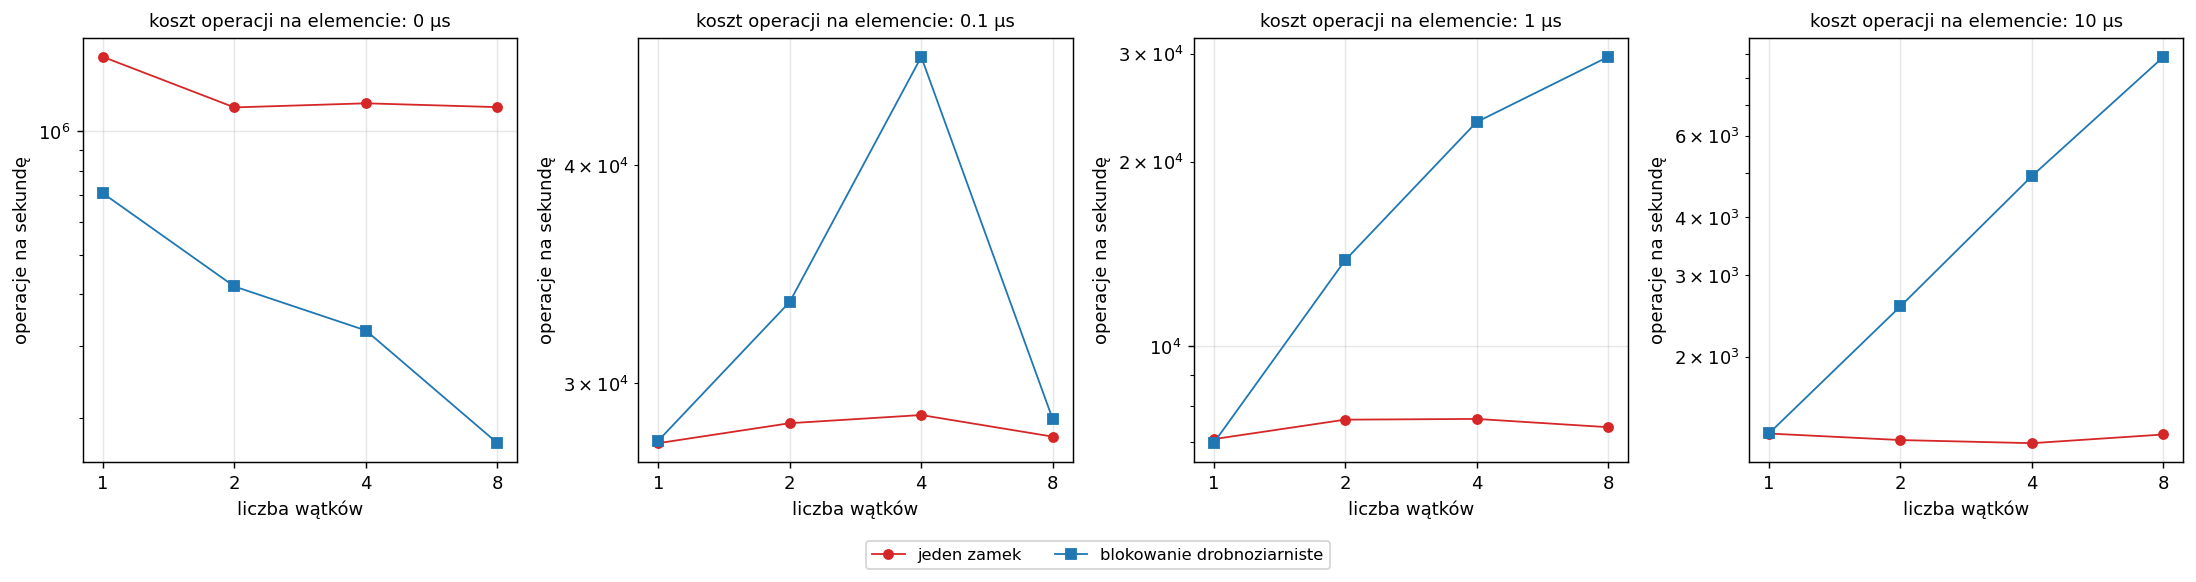
\includegraphics[width=\textwidth]{img/list.png}
    \caption{Przepustowość listy w zależności od liczby wątków i kosztu operacji na elemencie}
\end{figure}

\begin{table}[H]
    \centering
    \renewcommand{\arraystretch}{1.25}
    \begin{tabular}{|l|r|r|r|r|}
        \hline
        \textbf{Koszt operacji} & \textbf{1 wątek} & \textbf{2 wątki} & \textbf{4 wątki} & \textbf{8 wątków} \\ \hline
        0 \textmu s & \num{0.47} & \num{0.37} & \num{0.28} & \num{0.15} \\ \hline
        0,1 \textmu s & \num{1.00} & \num{1.17} & \num{1.60} & \num{1.02} \\ \hline
        1 \textmu s & \num{0.99} & \num{1.82} & \num{3.05} & \num{4.01} \\ \hline
        10 \textmu s & \num{1.00} & \num{1.94} & \num{3.78} & \num{6.54} \\ \hline
    \end{tabular}
    \caption{Przyspieszenie listy drobnoziarnistej względem listy z jednym zamkiem}
\end{table}

Lista z jednym zamkiem nie skaluje się: niezależnie od liczby wątków w liście pracuje tylko jeden,
więc jej przepustowość jest stała (np. 7062--7620 operacji na sekundę dla kosztu 1 \textmu s).
Bez kosztu operacji (0 \textmu s) lista drobnoziarnista jest wolniejsza: 2,1 raza przy jednym wątku
(zamknięcie i otwarcie zamka na każdym węźle kosztuje więcej niż samo porównanie) i 6,6 raza przy
8 wątkach, bo wątki stoją jeden za drugim w kolejce do zamków przy początku listy.
Dla kosztu 0,1 \textmu s zysk jest niewielki (najwyżej 1,60 raza dla 4 wątków).
Gdy operacja na elemencie jest droga, lista drobnoziarnista skaluje się prawie liniowo:
dla 10 \textmu s przyspieszenie wynosi 1,94, 3,78 i 6,54 raza dla 2, 4 i 8 wątków.
Wątki przechodzą listę jak potok -- każdy pracuje na innym węźle, a zamki są trzymane krótko
w porównaniu z kosztem operacji. Przyspieszenie nie osiąga liczby wątków, bo wątki nie mogą się
wyprzedzać, a 4 z 10 rdzeni procesora to szybsze rdzenie wydajnościowe, więc wolniejszy wątek
spowalnia wszystkie, które idą za nim.

\subsection{Wnioski}
Blokowanie drobnoziarniste opłaca się, gdy operacja na elemencie kosztuje znacznie więcej niż
zamknięcie i otwarcie zamka. Wtedy wiele wątków pracuje jednocześnie na różnych fragmentach listy
i przepustowość rośnie z liczbą wątków (6,5 raza dla 8 wątków i kosztu 10 \textmu s). Gdy operacja
jest tania, koszt zamków na każdym węźle dominuje i jedna blokada całej listy jest kilka razy szybsza.
Rozwiązanie jest też trudniejsze do poprawnego zaimplementowania niż jeden zamek.

\begin{thebibliography}{9}
    \bibitem{rw} \url{https://home.agh.edu.pl/~funika/tw/lab6/RW-problem.pdf}
    \bibitem{herlihy} M. Herlihy, N. Shavit: \textit{The Art of Multiprocessor Programming}, rozdz. 9 (Linked Lists: The Role of Locking). Morgan Kaufmann, 2012.
    \bibitem{downey} A. B. Downey: \textit{The Little Book of Semaphores}, rozdz. 4.2 (Readers-writers problem). 2016.
    \bibitem{jcu} \url{https://docs.oracle.com/en/java/javase/27/docs/api/java.base/java/util/concurrent/locks/Condition.html}
\end{thebibliography}

\end{document}
